\chapter{Prototyping Platform: Programmable Storage}
\label{chp:prototyping-platform}

\section{Ceph: A Distributed Storage System }
Ceph~\cite{weil:osdi2006-ceph} is a distributed storage platform that stripes
and replicates data across a reliable object store, called RADOS. Clients talk
directly to object storage daemons (OSDs) on individual disks. This is done by
calculating the data's placement (``where should I store my data") and location
(``where did I store my data") using a hash-based algorithm (CRUSH). This
architecture lets Ceph leverage the resources in the entire system because
individual OSDs manage the state of the system. 

CephFS is the POSIX-compliant file system that uses RADOS. CephFS is an
important part of the storage ecosystem because it acts as a gateway to the
file-based storage for legacy applications. It decouples metadata and data
access, so data IO is done directly with RADOS while all metadata operations go
to a separate metadata cluster. This metadata cluster exposes a hierarchical
namespace to the user using a technique called dynamic subtree
partitioning~\cite{weil:sc2004-dyn-metadata}. In this scheme, each metadata
server (MDS) manages a subtree in the namespace. 

The MDS cluster is connected to the clients to service metadata operations and
to RADOS so it can periodically flush its state. The CephFS components,
including RADOS, the MDS cluster, and the logical namespace, are shown
Figure~\ref{ceph-arch}. 

\begin{figure*}[tbh]
\centering
	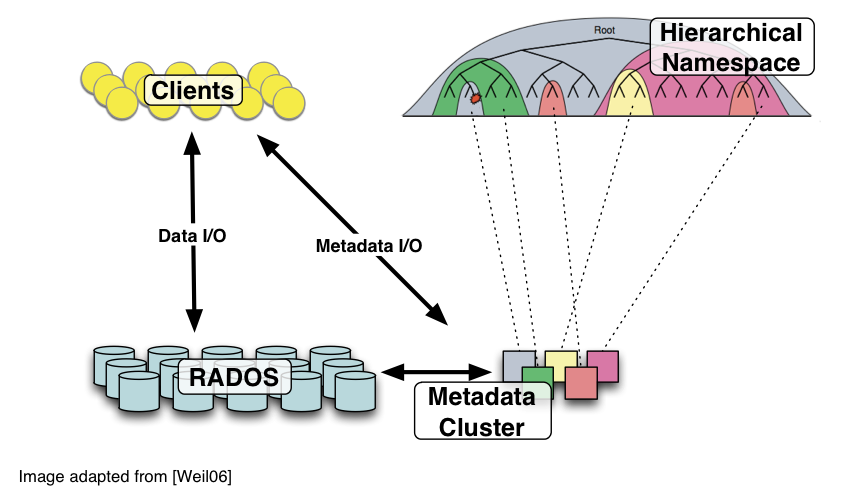
\includegraphics[width=1\textwidth]{./chapters/advancement/figures/ceph-arch.png} 

	\caption{\textbf{MDS cluster}: in CephFS, the clients interact with a
        MDS cluster for all metadata operations. The MDS cluster exposes a hierarchal
        namespace using a technique called dynamic subtree partitioning, where each MDS
        manages a subtree in the namespace.\label{ceph-arch}}

\end{figure*}

\subsection*{Why Use CephFS?}
\label{background-why}

CephFS has one of the most advanced metadata infrastructures and we use it as a
prototyping playform because (1) it was built for locality, (2) the migration
tools are already implemented, and (3) the system is highly available. 

% Locality
CephFS accommodates the locality in file systems by packaging related data
together. For example, inodes are embedded in directories so that related
inodes are fetched on a \texttt{readdir}. We predict that migration is fast
because directories are small. This is a consequence of having little
allocation metadata, since data location is calculated. 

% Implemented There are two problems with this approach: (1) the system is
% purely reactive, since data is moved when a certain event hits a threshold
% and (2) it doesn't have a good heuristic for where to move data. 
CephFS also has many migration features already implemented, most notably
directory migration and hotspot detection, as shown in Figure~\ref{ceph-arch}.
Ceph has the ability to move subtrees to different metadata servers
dynamically. Traditionally, when many creates/writes are made in the same
directory, the filenames are hashed across multiple metadata servers. When many
reads/opens are made to the same file, the contents are replicated across
different metadata servers. CephFS also other infrastructure already in-place,
such as: 

\begin{itemize}

\item ``\textbf{soft state}" for locating metadata: each MDS is only aware of
the metadata in its own cache so clients hop around the MDS cluster and
maintain their own hierarchical boundaries.

\item \textbf{replication} for distribution/high read availability: distributed
cache constraints allow path traversal to start at any node and to be
redirected upon encountering a subtree bound.

\item \textbf{locking} to maintain consistency: replicas are read-only and all
updates are forwarded to the authority for serialization/journaling; each
metadata field is protected by a distributed state machine.

\item \textbf{counters} to identify popularity: each inode and directory
fragment maintain a popularity vector to aid in load balancing; MDSs share
their measured loads so that they can determine how much to offload and to who
to offload to (favors reuniting parents with children). 

\item ``\textbf{frag trees}" for throughput (i.e. large directories): interior
vertices split by powers of two and directory fragments are stored as a
separate objects

\item ``\textbf{traffic control}" for flash crowd distribution (i.e.
simultaneous clients): MDS tells clients if metadata is replicated or not so
they can either contact the authority or replicas.

\end{itemize}

Moving the trees entails moving the subtree's cached metadata. It is performed
as a two-phase commit: importer journals metadata (Import event), exporter logs
event (Export event), importer journals event (ImportFinish). 

% Availabile
We use CephFS to explore the metadata management problem.
Finally, the Ceph system is accessible, active, and available. The source code
is open source under the GNU license and the community is very active. It was
also developed here at UC Santa Cruz, so it holds a special place in our heart.
Initial interactions with Inktank, the company delivers and supports Ceph, have
been positive, providing useful feedback and guidance. 
